\section{Tangent Spaces}
Lead question: ``What is the velocity of a curve $\gamma : \R \to M$ at the point $p$ of the curve in $M$?''

\subsection{Velocities}
% \url{https://youtu.be/pepU_7NJSGM?t=1m30s}
\begin{definition} Let $\mfd$ be a smooth manifold. Let there be a curve $\gamma : \R \to M$, which is at least $C^1$. Suppose $\gamma(\lambda_0) =p$. The \textbf{velocity} of $\gamma$ at the point $p$ of the curve $\gamma$ is the linear map \\
\begin{equation}\label{eq_velocity}
v_{\gamma, p} : C^{\infty}(M) \linearmapto \R \text{ with }
f \mapsto v_{\gamma,p}(f):= (f \after \gamma)^{\prime}(\lambda_0)
\end{equation}
where $C^{\infty}(M) := \lbrace f: M \to \R \, | \, f \text{ is a smooth function } \rbrace$ equipped with \\
$(f \oplus g)(p) := f(p) + g(p)$ and $(\lambda \otimes g)(p) := \lambda \cdot g(p)$ is a vector space.
\end{definition}

\begin{SCfigure}[5][h]
\label{fig:L5_fAfterGamma}
  \centering
	\begin{tikzpicture}
	  \matrix (m) [matrix of math nodes, row sep=4em, column sep=6em, minimum width=2em]
	  {
		\R & M & \R \\
	  };
	  \path[->]  
	  (m-1-1) edge node [auto] {$\gamma$} (m-1-2)
	          edge [bend right=30] node [auto] {$f \after \gamma$} (m-1-3)
	  (m-1-2) edge node [auto] {$f $} (m-1-3);
	\end{tikzpicture}
    \caption{$f \after \gamma$. Intuition: If the first $\R$ is thought of as time, and $f$ as temperature, then $f \after \gamma$ relates time and temperature and $(f \after \gamma)^\prime$ is the rate of change of temperature as you run around the curve.}
\end{SCfigure}

\underline{past}: `` $\underbrace{v^i}_{\text{vector in past}} (\partial_i f) = (\underbrace{v^i \partial_i}_{\text{vector as map}})f$ \\
\textit{In an imprecise way, we could say that we want vectors to survive as the directional derivatives they induce. This is a very slight shift of perspective which is extremely powerful and leads to idea of tangent space in differential geometry.}

\underline{Terminology}: If $X$ is a vector seen as a map, then $X$ acting on a function $f$, i.e. $Xf$ is called the \textbf{directional derivative of $f$ in the $X$ direction}.

\subsection{Tangent vector space}
% \url{https://youtu.be/pepU_7NJSGM?t=9m9s}
\begin{definition}
For each point $p \in M$, the \textbf{tangent space} to $M$ at the point $p$ is the set \\
\begin{equation}\label{Eq:L5_defTangentSpace}
T_p M := \lbrace v_{\gamma, p} \, | \, \text{ for all smooth curves } \gamma \text{ through } p \rbrace
\end{equation}
\end{definition}

\begin{SCfigure}[5][h]
\label{fig:L5_TangentPlane}
  \centering
    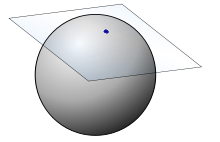
\includegraphics[width=0.3\textwidth]{5_Tangent_plane}
    \caption{A pictorial representation of the tangent space $T_xM$ of a single point, x, on a manifold. A vector in this $T_xM$ can represent a possible velocity at x. After moving in that direction to a nearby point, one's velocity would then be given by a vector in the tangent space of that nearby point — a different tangent space, not shown. \textit{By Alexwright at English Wikipedia - Transferred from en.wikipedia to Commons by Ylebru., Public Domain \url{https://commons.wikimedia.org/w/index.php?curid=3941393}}}
\end{SCfigure}

\begin{SCfigure}[5][h]
\label{fig:L5_TangentVector}
  \centering
    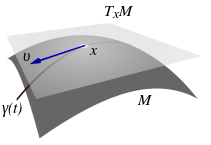
\includegraphics[width=0.3\textwidth]{5_Tangential_vector}
    \caption{The tangent space $T_xM$ and a tangent vector $v \in T_xM$, along a curve travelling through $x \in M$. \textit{By derivative work: McSush (talk)Tangentialvektor.png: TNThe original uploader was TN at German Wikipedia - Tangentialvektor.png, Public Domain, \url{https://commons.wikimedia.org/w/index.php?curid=4821938}}}
\end{SCfigure}

\textit{\textbf{Caution}: Although the Fig. \ref{fig:L5_TangentPlane} and \ref{fig:L5_TangentVector} refer to an ambient space in which $M$ is embedded, the tangent space has been defined intrinsically. There is a velocity corresponding to each curve along a different path in $M$ passing through $p$. Velocity along two different curves could be same, or curves along same paths but having different parameter speeds would yield different velocities.}

\begin{theorem}
$(T_pM, \oplus, \otimes)$ is a vector space with 
\begin{align*}
  \oplus : & T_pM \times T_pM \to Hom(C^\infty(M),\R)  \\
  & (v_{\gamma,p} \oplus v_{\delta,p})(\underbrace{f}_{ \in C^{\infty}(M)} ) := v_{\gamma,p}(f) +_{\R} v_{\delta,p}(f) \\
  \odot : & \R \times T_pM \to Hom(C^{\infty}(M),\R) \\
  & (\alpha \odot v_{\gamma,p} )(f) := \alpha \cdot_{\R}  v_{\gamma, p}(f)
\end{align*}
\end{theorem}

\begin{proof} Various conditions that must be satisfied by a vector space, are trivially satisfied. It remains to be shown that 
\begin{enumerate}[i)]
  \item For product, $\exists \, \tau $ curve : $\alpha \odot v_{\gamma,p} = v_{\tau,p}$
  \item For sum, $\exists \, \sigma$ curve : $v_{\gamma,p} \oplus v_{\delta,p} = v_{\sigma,p}$
\end{enumerate}
\underline{Product}: Let $\tau : \R \to M$ with $\lambda \mapsto \tau(\lambda) := \gamma(\alpha  \lambda + \lambda_0) = (\gamma \after \mu_{\alpha})(\lambda)$
where $\mu_{\alpha} : \R \to \R$ with $r \mapsto \alpha \cdot r + \lambda_0$. Then $\tau(0) = \gamma(\lambda_0) = p$, and
\[
v_{\tau,p} = (f \after \tau)^{\prime}(0) = (f \after \gamma \after \mu_{\alpha})^{\prime}(0) = \mu_{\alpha}^{\prime}(0) \cdot (f \after \gamma)^{\prime}(\mu_{\alpha}(0)) = \alpha \cdot (f \after \gamma)^{\prime}(\lambda_0) = \alpha \cdot v_{\gamma,p}
\]

\underline{Sum}: Choose a chart $(U,x)$ and $p \in U$. \textit{(If the proof will depend on the choice of a chart, alarm bells should ring. But we shall see that the result is finally independent of the chart.)} \\
Let $p = \gamma(\lambda_0) = \delta(\lambda_1)$. \\
Now define $\sigma : \R \to M$ with $\lambda \mapsto \sigma(\lambda) := x^{-1}(\underbrace{(x \after \gamma)(\lambda_0 + \lambda)}_{\R \to \R^d} + (x \after \delta)(\lambda_1 + \lambda) - (x \after \gamma)(\lambda_0))$. \\
Then, $\sigma_x(0) = x^{-1}((x \after \gamma)(\lambda_0) + (x \after \delta)(\lambda_1) - (x \after \gamma)(\lambda_0)) = \delta(\lambda_1) = p$. \\
Now
\begin{align*}
  v_{\sigma_x,p}(f) & := (f \after \sigma_x)^{\prime}(0) \\ 
  & = ( \underbrace{(f \after x^{-1})}_{\R^d \to \R} \after \underbrace{(x \after \sigma_x)}_{\R \to \R^d})^{\prime}(0) \\
  & = \underbrace{(x \after \sigma_x)^{\prime}(0)}_{(x \after \gamma)^{\prime}(\lambda_0) + (x \after \delta)^{\prime}(\lambda_1)} \cdot \left( \partial_i (f \after x^{-1}) \right)(x(\underbrace{\sigma(0)}_{p})) \\
  & = (x \after \gamma)^{\prime}(\lambda_0)(\partial_i (f \after x^{-1}))(x(p)) + (x \after \delta)(\lambda_1)(\partial_i (f \after x^{-1}))(x(p)) \\
  & = (f \after \gamma)^{\prime}(\lambda_0) + (f \after \delta)^{\prime}(\lambda_1) \\
  & = v_{\gamma,p}(f) + v_{\delta,p}(f) && \forall \, f \in C^{\infty}(M)
\end{align*}
\end{proof}

\underline{picture}: (cf. \url{https://youtu.be/pepU_7NJSGM?t=39m5s})

\textit{If we push $\gamma$ and $\delta$ to one chart, and add them there, then bring the sum back to $M$, we would get a curve which would be different from the curve we would get if we used another chart. But it turns out, irrespective of the charts selected, we get the same tangent/velocity. Conclusion: Adding trajectories is chart dependent; hence, bad. Adding velocities is good because, whatever the charts, they yield the same derivative at the point of intersection. Of course, you cannot add two curves $(\gamma \oplus \delta)(\lambda) := \gamma(\lambda) +_M \delta(\lambda)$ because there is no addition $+_M$ in $M$. Defining $+$ through charts results in chart-dependent results, which is, therefore, not real.}  

\subsection{Components of a vector w.r.t. a chart}
\begin{tikzpicture}
  \matrix (m) [matrix of math nodes, row sep=4em, column sep=6em, minimum width=2em]
  {
    \R & M & \R \\
    & \R^d & \\
  };
  \path[->]
  (m-1-1) edge node[auto] {$\gamma$} (m-1-2)
          edge node[sloped, anchor=center, below] {$x \after \gamma$} (m-2-2)
  (m-1-2) edge node[auto] {$x$} (m-2-2)
          edge node[auto] {$f$} (m-1-3)
  (m-2-2) edge node[sloped, anchor=center, below] {$f \after x^{-1}$} (m-1-3);
\end{tikzpicture}

Let $(U,x) \in \A_{\text{smooth}}, \, \gamma : \R \to U$ and $\gamma(0) = p$. Then
\begin{align*}
  v_{\gamma,p}(f) & := (f \after \gamma)^\prime(0) \\
  & = (\underbrace{(f \after x^{-1})}_{\R^d \to \R} \after \underbrace{(x \after \gamma)}_{\R \to \R^d})^\prime(0) \\
  & = \displaystyle\left(\left(x \after \gamma\right)^\prime\right)^i(0) \cdot \left(f \after x^{-1}\right)^\prime_i(x(p)) \\
  & = \underbrace{\displaystyle\left(\left(x \after \gamma\right)^\prime\right)^i(0)}_{=: \dot{\gamma}_x^i(0)} \cdot \underbrace{(\partial_i(f \after x^{-1}))(x(p))}_{=: \left(\cibasis[f]{x^i}\right)_p} \\
  & = \dot{\gamma}_x^i(0) \cdot \left(\cibasis{x^i}\right)_p f && \forall \, f \in C^{\infty}(M), f : M \to \R
\end{align*}

\begin{definition}
For velocity $v_{\gamma,p}$, as a map under use of a chart $(U,x)$,
\begin{equation}\label{eq:defVelocityExpansion}
\boxed{v_{\gamma,p} = \dot{\gamma}_x^i(0) \cdot \left(\cibasis{x^i}\right)_p}
\end{equation} 
where
\begin{equation}\label{eq:defVelocityComponents}
\displaystyle\dot{\gamma}_x^i = \left(\left(x \after \gamma\right)^\prime\right)^i
\end{equation} 
are the \textbf{components of the velocity} $v_{\gamma,p}$ and
\begin{equation}\label{eq:defCIBasis}
\displaystyle\left(\cibasis{x^i}\right) = \partial_i\left(\,\cdot \after x^{-1}\right) = \left(\left(\, \cdot \after x^{-1}\right)^\prime\right)^i
\end{equation} 
which eat a function, form a basis of $T_pM$ w.r.t. which the components of the velocity need to be understood.
\end{definition}

\textit{Note: The components of a vector are always w.r.t. a chart. In $M$, there is just the vector, no components.} \\
Picture: \url{https://youtu.be/pepU_7NJSGM?t=1h16s}

\begin{theorem}
\label{thm:L5_dxiupondxj}
For a chart $(U,x)$,
\begin{equation}
\boxed{\cibasis[x^i]{x^j} = \delta^i_j}
\end{equation}
\end{theorem}
\begin{proof}
\begin{align*}
\cibasis[x^i]{x^j} & = \partial_j (x^i \after x^{-1})(x(p)) \\
& = \delta^i_j && \text{ since } x^i \after x^{-1} : \R^d \to \R \text{ s.t. } (\alpha^1 , \dots , \alpha^d) \mapsto \alpha^i
\end{align*}
\end{proof}

\subsection{Chart-induced basis}
% \url{https://youtu.be/pepU_7NJSGM?t=1h2m}
\begin{definition}
If $(U,x) \in \A_{\text{smooth}}$, then $\displaystyle\left(\cibasis{x^1}\right)_p, \dotsc, \left(\cibasis{x^d}\right)_p \in T_pU \subseteq T_pM$ constitute a \textbf{chart-induced basis} of $T_pU$.
\end{definition}

\begin{proof} We have already shown that any vector in $T_pU$ can be expressed in terms of $\displaystyle\left(\cibasis{x^i}\right)_p$. It remains to be shown that they are linearly independent. That is, we require $\displaystyle\lambda^i \left(\cibasis{x^i}\right)_p = 0 \implies \lambda^i = 0$ for all $i = 1, \dotsc, d$. Or,
\begin{align*}
0 & = \lambda^i \left(\cibasis{x^i}\right)_p(x^j) && x^j : U \to \R \text{ is differentiable}\\
& = \lambda^i \partial_i (x^j \after x^{-1})(x(p)) && \text{by Eq. \ref{eq:defCIBasis}} \\
& = \lambda^i \delta^j_i && \text{by Theorem \ref{thm:L5_dxiupondxj}} \\
& = \lambda^j && \text{for all } j = 1, \dotsc, d 
\end{align*}
\end{proof}

\begin{corollary}
$dim \, T_pM = d = dim \, M$. \\
This follows from the fact $d$ vectors are needed to express any vector in $T_pM$, and these $d$ vectors arise from the $d$ coordinates of chart which shows that $M$ has $d$ dimensions.
\end{corollary}

\underline{Terminology}: $X \in T_pM \implies \exists \, \gamma : \R \to M : X = v_{\gamma,p}$ and $\displaystyle \exists \, \underbrace{X^1, \dotsc, X^d}_{\in \R} : X = X^i \left(\cibasis{x^i}\right)_p$. $X^i$ are called \textbf{components of the vector $X$ w.r.t chart-induced basis}.

\subsection{Change of vector components under a change of chart}
\ding{56} A vector does not change under change of chart. It is the vector components that transform under a change of chart.

Let $(U,x)$ and $(V,y)$ be overlapping charts and $p \in U \cap V$. Let $X \in T_pM$. Then, $X$ can be expanded in terms of chart-induced basis of the two charts as follows:
\begin{equation}\label{eq:L5_VecExpandedIn2Charts}
X^i_{(y)} \cdot \left(\cibasis{y^i}\right)_p \underbrace{=}_{(V,y)} X \underbrace{=}_{(U,x)} X^i_{(x)} \cdot \left(\cibasis{x^i}\right)_p
\end{equation}
Now,
\begin{align*}
  \left(\cibasis{x^i}\right)_p f & = \partial_i(f \after x^{-1})(x(p)) \\
  & = \partial_i (\underbrace{(f \after y^{-1})}_{\R^d \to \R} \after (\underbrace{y \after x^{-1}}_{\R^d \to \R^d})(x(p)) \\
  & = (\partial_i (y \after x^{-1})^j)(x(p)) \cdot (\partial_j (f \after y^{-1}))(y(p)) \\
  & = (\partial_i (y^j \after x^{-1}))(x(p)) \cdot (\partial_j (f \after y^{-1}))(y(p)) \\
  & = \boxed{\left(\cibasis[y^j]{x^i}\right)_p \cdot \left(\cibasis[f]{y^j}\right)_p}
\end{align*}

\begin{equation}\label{eq:L5_cibasisIn2Charts}
\therefore \boxed{\left(\cibasis{x^i}\right)_p = \left(\cibasis[y^j]{x^i}\right)_p \cdot \left(\cibasis{y^j}\right)_p}
\end{equation}
Using Eq. \ref{eq:L5_VecExpandedIn2Charts} and Eq. \ref{eq:L5_cibasisIn2Charts}, 
\[
  X^i_{(x)} \left(\cibasis[y^j]{x^i}\right)_p \left(\cibasis{y^j}\right)_p = X^j_{(y)}\left(\cibasis{y^j}\right)_p
\]
\begin{equation}
\therefore \boxed{X^j_{(y)} = \left(\cibasis[y^j]{x^i}\right)_p X^i_{(x)}}
\end{equation}

\subsection{Cotangent spaces}
% \url{https://youtu.be/pepU_7NJSGM?t=1h24m36s}
Since $T_pM$ is a vector space, therefore it is trivial to define cotangent space as follows.

\begin{definition}
For the tangent space $T_pM$ at $p \in M$, \textbf{cotangent space} is defined as
\begin{equation}
(T_pM)^* := \lbrace \varphi : T_pM \linearmapto \R \rbrace
\end{equation}
\end{definition}

\begin{definition}
\label{def:gradient}
If $f \in C^{\infty}(M)$, then the \textbf{gradient of $f$ at the point $p \in M$} is defined as
\begin{align}
\label{eq:defGradient}
  (df)_p : & T_p M \linearmapto \R \nonumber \\ 
  & X \mapsto (df)_p(X) := Xf
\end{align}

\end{definition}
i.e. $\boxed{(df)_p \in T_pM^*}$

$(df)_p$ is a $(0,1)$-tensor over the underlying vector space $T_pM$. We define the components of the gradient the same way as we define the components of a tensor (refer section \ref{ss:L3_TensorComponents}).

\begin{definition}
\textbf{Components of gradient w.r.t. chart-induced basis of $(U,x)$} are defined as
\begin{equation}
\left((df)_p \right)_j := (df)_p\left(\left(\cibasis{x^j}\right)_p \right) = \left(\cibasis[f]{x^j}\right)_p = \partial_j (f \after x^{-1})(x(p))
\end{equation}
\end{definition}

\begin{theorem}
A chart $(U,x) \implies x^i : U \to \R$ are smooth functions. Then, $(dx^1)_p, (dx^2)_p, \dotsc, (dx^d)_p$ form a basis of $T_p^*M$. 
\end{theorem}

\begin{proof}
In fact, $(dx^i)_p$ form a dual basis since 
\begin{equation}
(dx^a)_p \left(\left(\cibasis{x^b}\right)_p \right) = \left(\cibasis[x^a]{x^b}\right)_p = \delta_b^a \textit{ (using Theorem \ref{thm:L5_dxiupondxj})}
\end{equation}
\end{proof}

\subsection{Change of components of a covector under a change of chart}
\ding{56} A covector does not change under change of chart. It is the covector components that transform under a change of chart.

Let $(U,x)$ and $(V,y)$ be overlapping charts and $p \in U \cap V$. Let $\omega \in T_p^*M$. Then, $\omega$ can be expanded in terms of chart-induced basis of the two charts as follows:
\begin{equation}\label{eq:L5_CovecExpandedIn2Charts}
\displaystyle\omega_{(y)j}(dy^j)_p \underbrace{=}_{(V,y)} \omega \underbrace{=}_{(U,x)} \omega_{(x)i}(dx^i)_p
\end{equation}

Now,
\begin{align*}
  && \displaystyle\omega_{(y)j}(dy^j)_p & = \omega_{(x)i}(dx^i)_p && \text{by Eq. \ref{eq:L5_CovecExpandedIn2Charts}} \\
  \implies && \displaystyle\omega_{(y)j}(dy^j)_p \left(\cibasis{y^k}\right)_p & = \omega_{(x)i}(dx^i)_p \left(\cibasis{y^k}\right)_p \\
  \implies && \displaystyle\omega_{(y)j}(dy^j)_p \left(\cibasis{y^k}\right)_p & = \omega_{(x)i}(dx^i)_p \left(\cibasis[x^q]{y^k}\right)_p \cdot \left(\cibasis{x^q}\right)_p && \text{by Eq. \ref{eq:L5_cibasisIn2Charts}} \\
  \implies && \displaystyle\omega_{(y)j} \left(\cibasis[y^j]{y^k}\right)_p & = \omega_{(x)i} \left(\cibasis[x^q]{y^k}\right)_p \cdot \left(\cibasis[x^i]{x^q}\right)_p && \text{by Eq. \ref{eq:defGradient}} \\
  \implies && \displaystyle\omega_{(y)j} \delta^j_k & = \omega_{(x)i} \left(\cibasis[x^q]{y^k}\right)_p \cdot \delta^i_q && \text{by Theorem \ref{thm:L5_dxiupondxj}} \\
  \implies && \displaystyle\omega_{(y)k} & = \omega_{(x)i} \left(\cibasis[x^i]{y^k}\right)_p
\end{align*}
Or, with a change of indices,
\begin{equation}
\boxed{\omega_{(y)i} = \left(\cibasis[x^j]{y^i}\right)_p \omega_{(x)j}}
\end{equation}

\begin{align*}
&& \omega_{(y)i} & = \left(\cibasis[x^j]{y^i}\right)_p \omega_{(x)j} \\
\implies && \omega_{(y)i}(dy^i)_p & = \left(\cibasis[x^j]{y^i}\right)_p \omega_{(x)j}(dy^i)_p \\
\implies && \omega & = \left(\cibasis[x^j]{y^i}\right)_p \omega_{(x)j}(dy^i)_p \\
\implies && \omega (dx^j)_p & = \left(\cibasis[x^j]{y^i}\right)_p \omega_{(x)j}(dy^i)_p (dx^j)_p \\
\implies && \omega (dx^j)_p & = \left(\cibasis[x^j]{y^i}\right)_p \omega (dy^i)_p \\
\implies && (dx^j)_p & = \left(\cibasis[x^j]{y^i}\right)_p (dy^i)_p
\end{align*}

\begin{equation}\label{eq:L5_cicobasisIn2Charts}
\therefore \boxed{(dx^j)_p = \left(\cibasis[x^j]{y^i}\right)_p (dy^i)_p}
\end{equation}
